Currently, the main problem in extracting the GW background is the high instrumental noise. Ground-based detectors today, like LIGO, Virgo \& KAGRA are not able to detect any GW background as discussed in section \ref{astro_GWB}. This is why we need future detectors such as Einstein Telescope (ET) or Cosmic Explorer (CE) to achieve a higher sensitivity.

\section{LIGO, Virgo \& KAGRA}

The current most sensitive GW observatory is LIGO in the United States, operating an interferometer with two arms, each 4 km long. The data is analysed jointly with the Virgo detector in Italy and KAGRA in Japan. This is very useful since it allows cross-correlation which lowers the noise level.

\begin{figure}[h]
    \centering
    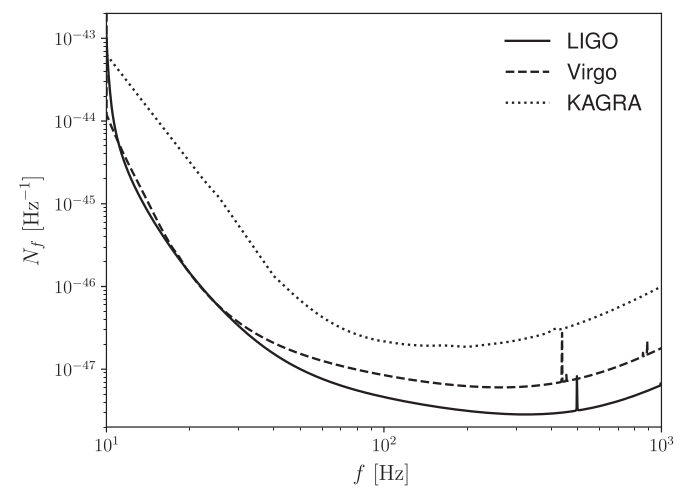
\includegraphics[width=7.5cm]{Images/lvk_frequency_noise.png}
    \caption[Noise sensitivity with respect to frequency for LVK.]{Design sensitivity curves for the LVK detector network. For LIGO, this is the advanced LIGO A+ design sensitivity and for Virgo the O5 sensitivity. This figure is taken from \cite{alonso_noise_2020}.}
    \label{lvk_frequency}
\end{figure}

\begin{figure}[h]
    \centering
        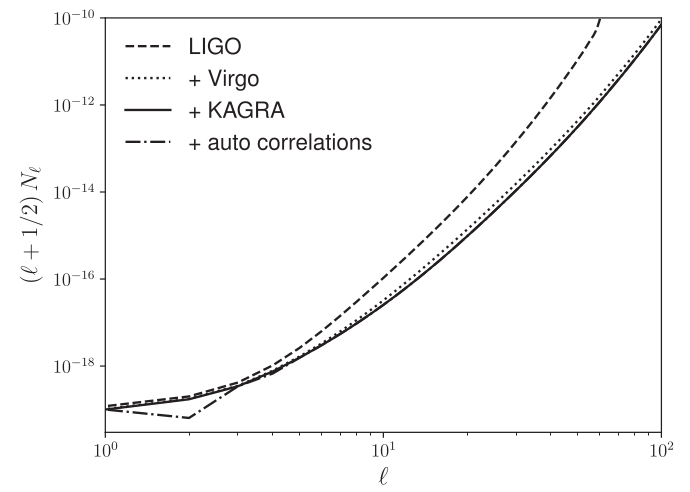
\includegraphics[width=7.5cm]{Images/alonso_ligo_noise.png}
    \caption{The noise angular power spectrum for LVK.}
    \label{lvk_Cl}
\end{figure} 

In Fig. \ref{lvk_frequency}, we see how the sensitivity changes with respect to the frequency. The most sensitive frequency range is at $100 -1000$ Hertz.
The noise power spectrum in Fig. \ref{lvk_frequ} tells us at which magnitude we could expect to measure a certain multipole.
As can be seen in Fig.\ref{lvk_Cl}, using cross-correlations between the ground-based detectors improves the sensitivity, especially at higher multipoles. Adding auto-correlations of the detectors mostly influences $\ell=2$, which is due to the L-shaped geometry of the detectors. 

\section{Einstein Telescope \& Cosmic Explorer}

\label{ET_CE}

ET will be a third-generation ground-based observatory, built either in the Limburg region in the Netherlands or in Sardinia in Italy. Its sensitivity will be vastly improved compared to LVK. This is due to the fact that it will operate in three arms with 10 km each instead of two arms measuring 4 km like LVK. A similar project is planned in the United States, called Cosmic Explorer (CE). It will have two arms with an unprecedented length of 40 km. The frequency sensitivity curves are shown in Fig. \ref{ET_sensitivity}.

\begin{figure}[h]
    \centering
    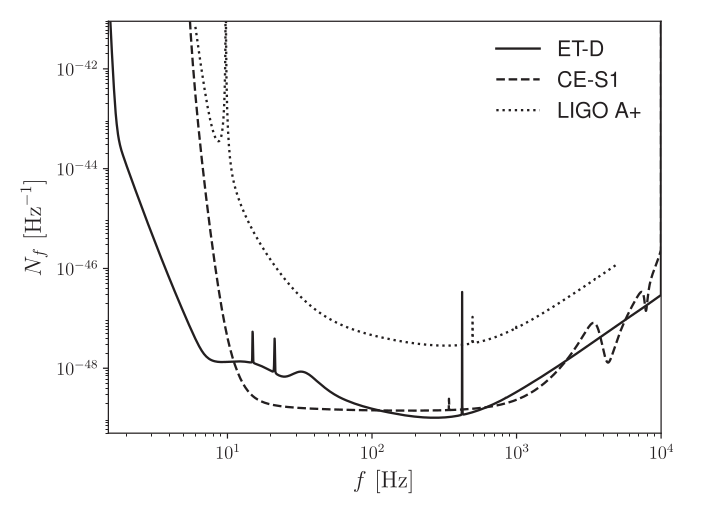
\includegraphics[width=0.7\linewidth]{Images/ET_CE_frequency_noise.png}
    \caption[The design sensitivity curve for ET and CE compared to LIGO A+.]{The design sensitivity curve for ET and CE compared to LIGO A+. This figure is taken from \cite{alonso_noise_2020}.}
    \label{ET_sensitivity}
\end{figure} 

ET and CE in cross-correlation will improve the sensitivity in the angular power spectrum by around 4 orders of magnitude, see Fig.\ref{ET_Cl}.  Here again, the improvement coming from the auto-correlation at $l=2, 4$ is due to the detector shape.

\begin{figure}[h]
    \centering
    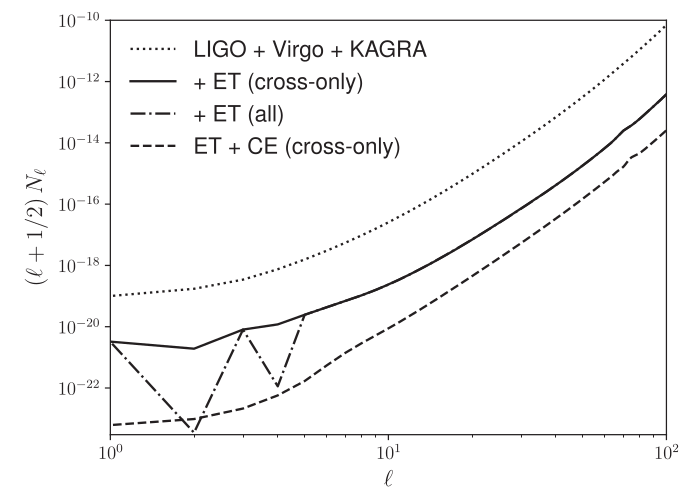
\includegraphics[width=0.7\linewidth]{Images/et_ce_Cl_noise.png}
    \caption[The noise angular power spectrum for different detectors at a reference frequency of 63 Hertz.]{The noise angular power spectrum for different detectors at a reference frequency of 63 Hertz. LVK a the dotted line, ET in solid and dot-dashed lines and CE in a dashed line. This figure is taken from \cite{alonso_noise_2020}.}
    \label{ET_Cl}
\end{figure} 

Using the cross-correlations between ET and CE, see Fig.\ref{ET_Cl}, the noise angular power spectrum is expected to drop from $10^{-19}$ to $\approx 6\cdot 10^{-24}$ for the dipole $\ell =1$.